\input{./_path-to-root.ltx}
\documentclass[\PathToRoot/\ProjectName]{subfiles}
\whenstandalone{\externaldocument{\PathToRoot/\ProjectName}}

\begin{document}

\begin{figure}[H]
  \centering
  \caption{Validation moments in models with and without splurge}
  \whenintegrated{\label{fig:untargetedMoments_wSplZero}} 
  \noindent\begin{minipage}{\textwidth}
    \centering
    \begin{subfigure}[b]{.48\linewidth}
      \centering
      \includegraphics[width=\linewidth]{\PathToRoot/images/iMPCs_both}
      \caption{Dynamic spending comparison}
      \whenintegrated{\label{fig:USaggmpclotterywin_wSplZero}} 
    \end{subfigure}
    %
    \begin{subfigure}[b]{.48\linewidth}
      \centering
      % Original path: \PathToRoot/Code/HA-Models/FromPandemicCode/Figures/Splurge0/UIextension_CompSplurge0
      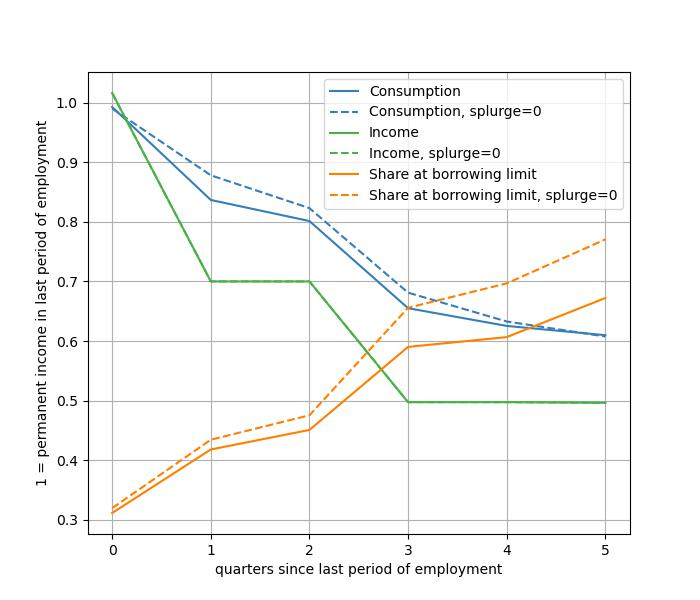
\includegraphics[width=\linewidth]{\PathToRoot/images/UIextension_CompSplurge0}
      \caption{UI benefit expiry dynamics}
      \whenintegrated{\label{fig:expiryUI_wSplZero}} 
    \end{subfigure}
  \end{minipage}
\end{figure}
\noindent\parbox{\textwidth}{\footnotesize
  \textbf{Note}: This figure validates both model variants against empirical evidence (Appendix~\ref{app:Model-without-splurge}).
  Subfigure~(a) compares dynamic consumption response to \cite{fagereng-mpc-2021} estimates;
  the no-splurge model shows slightly low MPC in year 1 and high MPC in year 2 due to
  faster spending by borrowing-constrained agents from the wider discount factor distribution.
  Subfigure~(b) shows UI benefit expiry dynamics compared to \cite{ganongConsumer2019};
  both models predict similar consumption drops (17\% vs.\ 18\%) when benefits expire,
  but through different mechanisms: direct splurge effects vs.\ increased borrowing constraints.
  Red lines show income dynamics, demonstrating model consistency across specifications.
}

\vspace{2em}  % Increase space after Figure 7 in appendix

% Smart bibliography: Only include bibliography if standalone AND has citations
\smartbib

\end{document}
